\section{Pogonski alat Unity}
Unity je softver koji pruža stvaraocima igara sve potrebne dodatke kako bi se omogućila što brža i efektivnija izrada igara.
Pogonski alat za igre (engl.~\textit{Game engine}) je razvojni okvir koji omogućava upotrebu 2D i 3D modela te slika iz drugih softvera kao što su Maya, Blender ili Photoshop.
Isto tako omogućava jednostavno sastavljanje svih važnih komponenti koje su potrebne za jednu igru, kao što su svjetlost, zvuk, specijalni efekti, fizika, animacije itd.
Rad u Unity možemo podijeliti na dva dijela. Jedan je rad unutar razvojnog okruženja Unity koji obuhvaća upotrebu svih mogućnosti pogonskog alata. Drugi dio je programiranje, odnosno razvijanje softvera koristeći Microsoft Visual Studio ako radite unutar operacijskog sustava Windows ili MonoDevelop unutar operacijskog sustava Linux.
U nastavku će biti opisan rad u jednom i u drugom dijelu.

Kada se govori o grafici, to podrazumijeva kvalitetnu arhitekturu sa sveukupnim mogućnostima vizualizacije visokih performansi kao i pristup brzo grafičkom sučelju, kako bi se omogućila što vjernija vizualna kvaliteta igre.

Zvuk se može stvarati i uređivati van okvira Unityja, odnosno koristeći aplikacije treće strane. Nakon toga se gotovi zvuk integrira u igru, bilo kao dio atmosfere, efekta određenih predmeta ili kao dio nekog događaja igre.

Jedna od najvažnijih komponenti pogonskog alata je fizika. Fizika je već integrirana u alat te uz samo nekoliko linija koda moguće je postići vjerodostojne efekte, odnosno ponašanje različitih objekata unutar igre. To omogućava dizajneru igre da manje vremena potroši na mukotrpno stvaranje fizike, a više na integriranje vlastitih ideja kako napraviti igru što zanimljivijom.

Isto tako omogućeno je jednostavno stvaranje grafičkog sučelja za samog igrača unutar igre, što uključuje različite izbornike, statistiku, kao i prikaz najvažnijih podataka tijekom igranja, kao što su rezultat, zdravlje, navigacijska karta itd.

Unity podržava programiranje u C\#, isto tako dolazi s određenim standardnim skriptama koje omogućuju korisniku brzi početak rada, te stvaranja prve igre bez previše kodiranja. Od velike pomoći su gotovi projekti koji se nalaze na stranicama Unityja te isto tako omogućuju jednostavno upoznavanje s procesom rada te ključnim segmentima izrada igara.

Unity je više-platformski što znači da se može koristiti, te se isto tako konačni produkt može prevesti i pokrenuti na različitim operacijskim sustavima. Omogućava izradu više vrsta projekata, to uključuje: 
\begin{itemize}
 \item Kompletna 3D igra,
 \item ortografska 3D igra,
 \item kompletan 2D,
 \item 2D način igranja s 3D grafikom,
 \item 2D način igranja i grafika, s kamerama različitih perspektiva.
\end{itemize}
 %Na preddiplomskom studiju je uglavnom predviđeno da student za praktični dio rada (analiza, prikupljanje zahtjeva, teoretsko istraživanje, izrada aplikacije) iskoristi 300 sati, a za samo pisanje i pripremu obrane preostalih 60 sati. Na specijalističkom studiju IT-a rad je vrednovan s 20 ECTS bodova što predstavlja 600 sati rada, tj.~predviđeno je da student za praktični dio rada (analiza, prikupljanje zahtjeva, teoretsko istraživanje, izrada aplikacije) iskoristi približno 420 sati, a za samo pisanje i pripremu obrane preostalih 180 sati.

U nastavku će biti prikazano sučelje preko slika te će isto tako biti opisane pojedinačne komponente. 

\subsection{Upoznavanje sa sučeljem}
Prije početka rada dobro je se upoznati s razvojnim sučeljem, glavni zaslon se može prilagoditi tako da si posložite glavne prozore za rad prema vlastitim sklonostima, to uključuje kompletnu promjenu rasporeda, dodavanje i uklanjanje različitih prozora i tabova. Glavni prozor je prikazan na slici~\ref{fig:Editor}.
\\[\intextsep]
\begin{minipage}{\linewidth}
\centering%
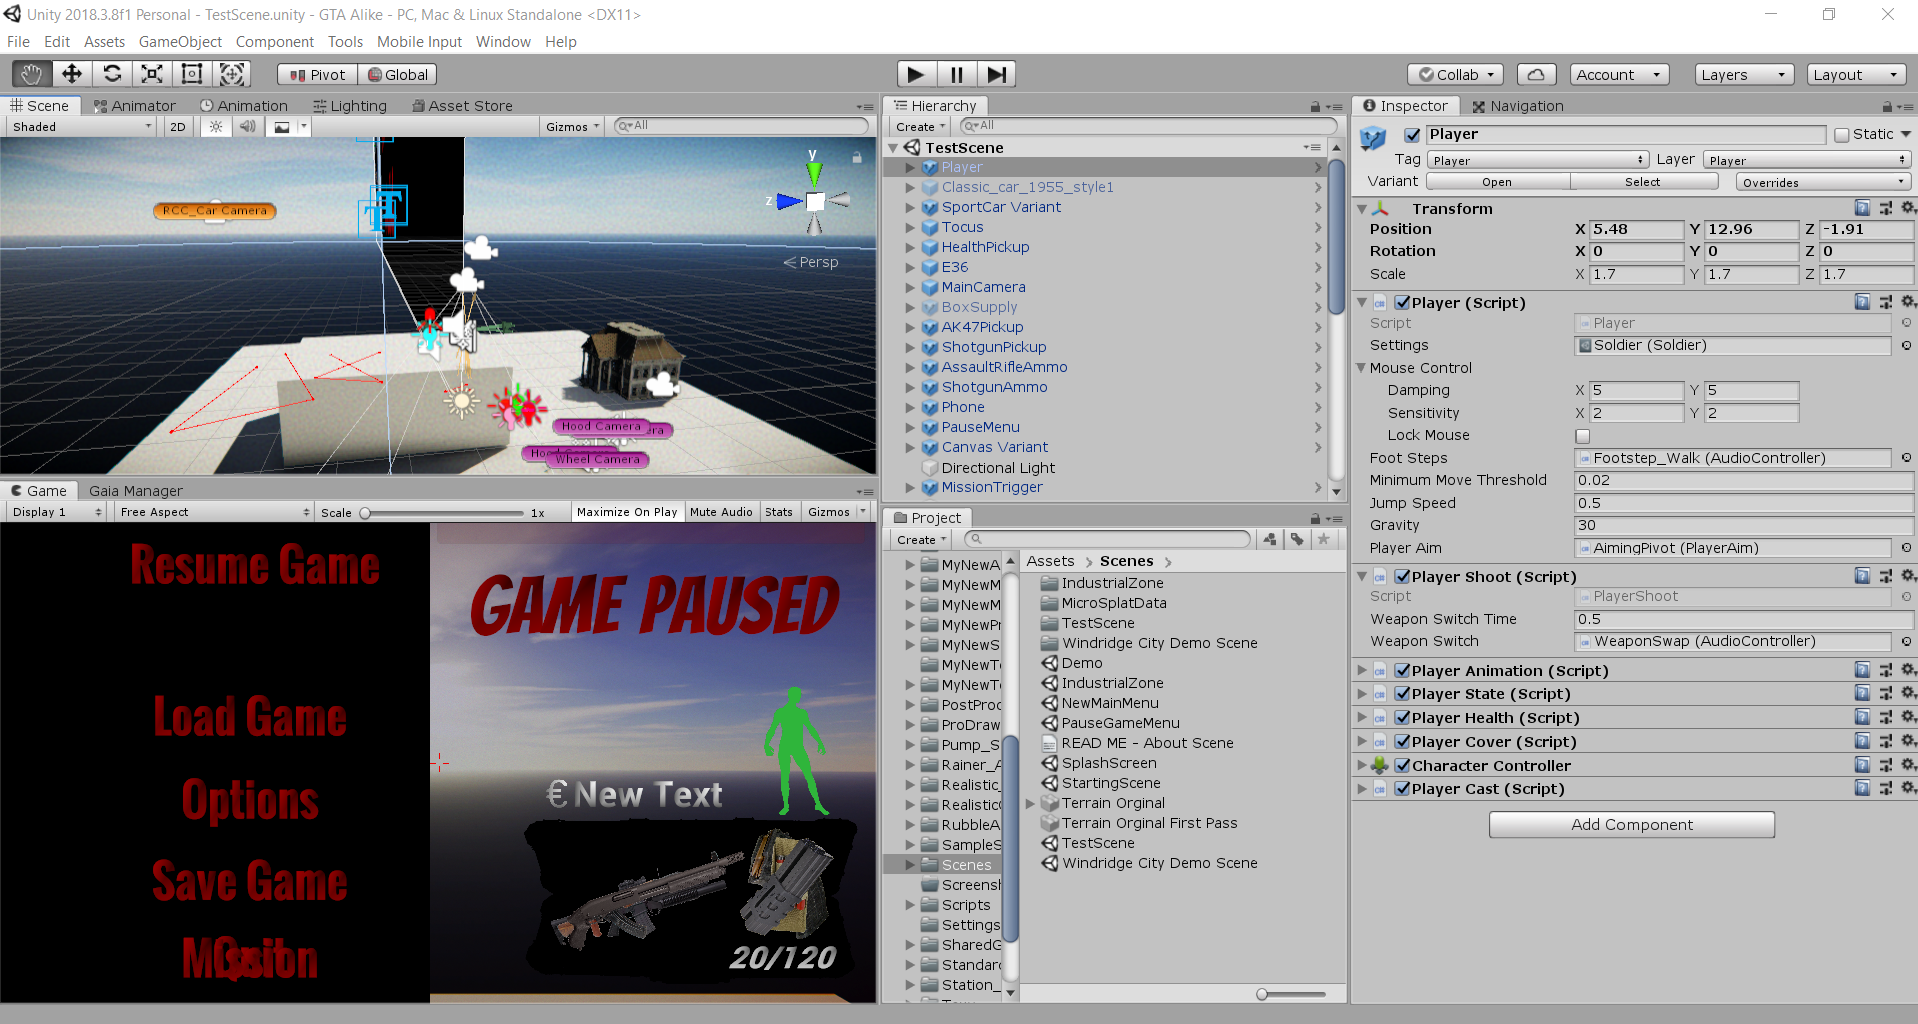
\includegraphics[width=0.6\linewidth,clip=]{slike/Editor.png}
\figcaption{Radno sučelje Unity}%
\label{fig:Editor}%
\end{minipage}
\\[\intextsep]

Glavni prozor uključuje:
\begin{itemize}
 \item Alatnu traku,
 \item prikaz scene,
 \item nadgledni prozor (engl.~\textit{Inspector window}),
 \item projektni prozor,
 \item hijerarhijski prikaz objekata.
\end{itemize}

Projektni prozor~\ref{fig:ProjectWindowCallout} prikazuje kompletnu biblioteku dodataka koji su dostupni u projektu.
Kada preuzmete dodatak sa stranica trgovine s dodacima (engl.~\textit{Asset store-a}), napravi se direktorij koji sadrži taj dodatak unutar ovog prozora.
\\[\intextsep]
\begin{minipage}{\linewidth}
\centering%
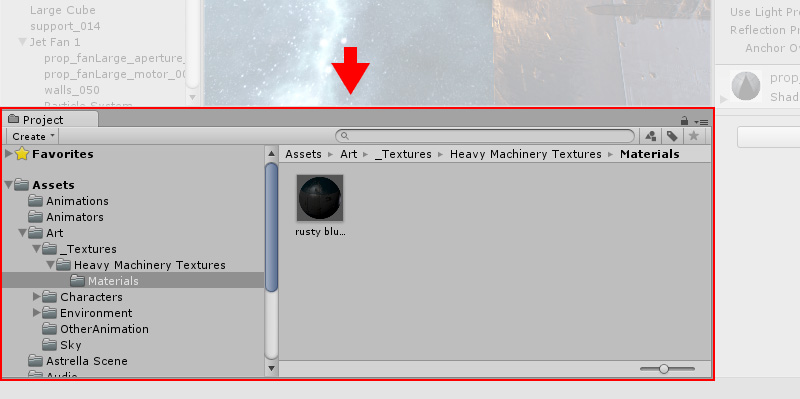
\includegraphics[width=0.6\linewidth,clip=]{slike/ProjectWindowCallout.jpg}
\figcaption{Projektni prozor}%
\label{fig:ProjectWindowCallout}%
\end{minipage}
\\[\intextsep]

Prikaz scene~\ref{fig:scene} je uz hijerarhijski prikaz, najkorišteniji prozor unutar samog sučelja. Omogućava pomicanje objekata, rotiranje, navigiranje po sceni itd. Moguće su 3D ili 2D perspektive ovisno o tome o kakvom se projektu radi, isto tako ovisno o tome radi li se grafičko sučelje za igru, odnosno HUD-u  (engl.~\textit{Head-up display}). Isto tako su u prikazu scene vidljive promjene osvijetljena ovisno o tome jesu li uključene postavke za to.
\\[\intextsep]
\begin{minipage}{\linewidth}
\centering%
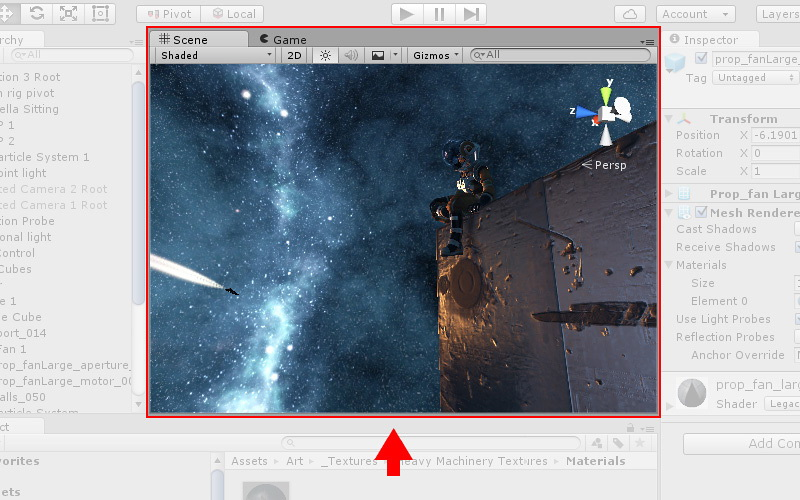
\includegraphics[width=0.4\linewidth,clip=]{slike/scene.jpg}
\figcaption{Prikaz scene}%
\label{fig:scene}%
\end{minipage}
\\[\intextsep]

Hijerarhijski prikaz~\ref{fig:HierarchyWindowCallout} je hijerarhijski tekstualni prikaz svakog objekta u sceni. Svaki objekt unutar scene se isto tako nalazi i u ovom prozoru, hijerarhija prikazuje kako su objekti međusobno povezani. Unutar ovog prozora moguće je preimenovati različite objekte, postavljati vidljivost, mijenjati raspored te naravno brisati i dodavati objekte unutar scene.
\\[\intextsep]
\begin{minipage}{\linewidth}
\centering%
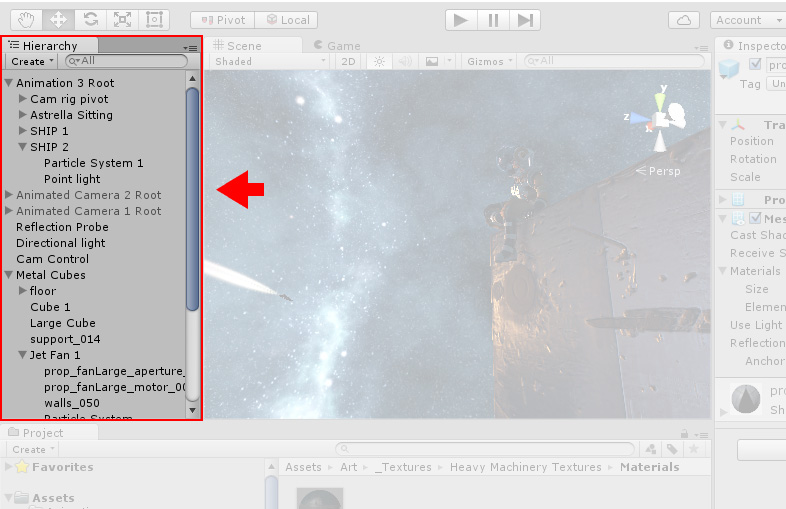
\includegraphics[width=0.6\linewidth,clip=]{slike/HierarchyWindowCallout.jpg}
\figcaption{Hijerarhijski prikaz}%
\label{fig:HierarchyWindowCallout}%
\end{minipage}
\\[\intextsep]

Nadgledni prozor~\ref{fig:inspector} omogućuje prikaz i promjenu svojstava trenutno izabranog objekta. Kako različiti objekti imaju različita svojstva, sami prikaz i sadržaj ovog prozora će se razlikovati ovisno o tome. Ovaj prozor se najviše koristi za promjenu položaja objekta unutar scena ako su poznate koordinate ili je potrebno fino pomicanje, isto tako služi za promjenu veličine objekta, kao i za dodavanje različitih komponenti kao što fizička svojstva, grafički prikaz, materijali te skripte.
\\[\intextsep]
\begin{minipage}{\linewidth}
\centering%
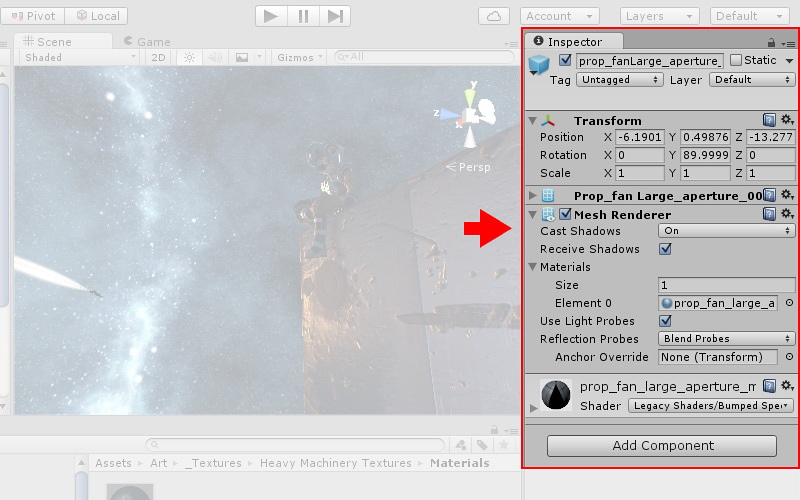
\includegraphics[width=0.4\linewidth,clip=]{slike/inspector.jpg}
\figcaption{Nadgledni prozor}%
\label{fig:inspector}%
\end{minipage}
\\[\intextsep]

Alatna traka~\ref{fig:ToolbarCallout} omogućava pristup najvažnijim komponentama za rad, na lijevoj strani se nalaze osnovni alati za upravljanje scenom i objektima unutar scene. U sredini su kontrole za pokretanje, stopiranje i pauziranje igre. Na desnoj strani se nalaze botuni koji omogućavaju pristup Unity računu i servisima unutar Unity oblaka (engl.~\textit{Unity Cloud Services}). Tu su još komande za promjenu prikaza sučelja te spremanje vlastitih postavki.
\\[\intextsep]
\begin{minipage}{\linewidth}
\centering%
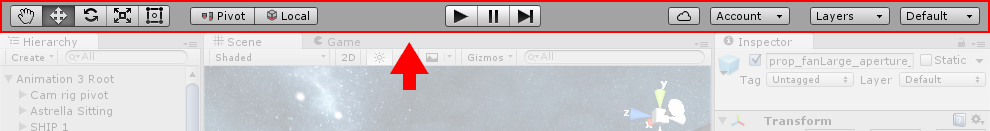
\includegraphics[width=0.6\linewidth,clip=]{slike/ToolbarCallout.png}
\figcaption{Alatna traka}%
\label{fig:ToolbarCallout}%
\end{minipage}
\\[\intextsep]

\subsection{Rad s dodacima}
Dodaci (engl.~\textit{Assets}) su svi elementi koji se mogu koristiti unutar projekta. To mogu biti modeli, audio datoteke, slike, ili bilo koje druge datoteke koja se može koristiti unutar Unityja. Osim toga postoje dodaci koji se mogu kreirati unutar Unity, kao što su kontroler animacije (engl.~\textit{Animator controller}), mikser zvukova (engl.~\textit{Audio mixer}) učitavač tekstura (engl.~\textit{Render texture}).
U nastavku će kratko biti navedeno te opisano što Unity podržava i koja je svrha određenih dodataka.

Unity podržava sve standardne formate slika kao što su BMP, TIF, JPG, PNG kao i sve standardne formate audio datoteka.
Kada je riječ o modelima, uglavnom se radi o FBX formatu datoteka, u slučaju da korisnik spremi datoteka u drugom formatu ona se uvozi u Unity kao FBX datoteka.
Standardni dodaci koji dolaze s Unity su uglavnom elementi, odnosno skripte koje se koriste uglavnom u svim projektima kao što su:
\begin{itemize}
 \item Postavke kamere,
 \item određeni likovi,
 \item više-platformski unos,
 \item efekti i okolina,
 \item sistem čestica,
 \item vozila.
\end{itemize}

Kao što postoje primitivni tipovi u programskim jezicima tako postoje određeni primitivni objekti unutar Unityja. To su:
\begin{itemize}
 \item Kocka, koja osim što predstavlja kocku, kada se rastegne može predstavljati i zidove, okidače, kao i privremeni držač za neki objekt.
 \item Kugla, osim logične upotrebe kao što su planet,lopta i slično može se koristiti npr. kao prikaz radijusa nekog efekta.
 \item Kapsula, najčešće služi kao privremeni držač za neki objekt.
 \item Valjak,
 \item ravnina, služi uglavnom kao ravna površina, pod ili zid.
 \item Četverokut, za prikaz slika i slično.
\end{itemize}

Kada je riječ o korištenju kompletno izrađenih dodataka od strane neke treće osobe, odnosno projekata koji se nalaze u trgovini za dodatke. Na stranicama trgovine (engl.~\textit{Asset store}) nalazi se mnoštvo projekata, bilo različitih modela, potrebnih mehanizama u igri, skripti koje olakšavaju izradu različitih komponenti igre, kao i kompletne igre koje mogu biti korištene unutar vlastitog projekta. Neki projekti su besplatni, dok je neke, vjerojatno kvalitetnije potrebno kupiti. Međutim čak i upotrebom besplatnih mogu se napraviti odlične igre. Unutar Dionyzus igre korišteni su isključivo besplatni dodaci.
Dodatak se prvo skine na računalo te nakon toga uvozi u projekt, mogu se uvesti samo potrebni dijelovi te u slučaju potrebe nadograditi. Isto tako je moguće izvoziti vlastite dodatke, tako što napravite vlastiti paket za izvoz.

